%%%%%%%%%%%%%%%%%%%%%%%%%%%%%%%%%%%%%%%%%%%%%%%%%%%%%%%%%%%%%%%%%%%%%%%%%
% This file is part of the LaTeX sources of the OMDoc 1.6 project descriptions
% Copyright (c) 2006 Andreas Franke, Michael Kohlhase
% This work is licensed by the Creative Commons Share-Alike license
% see http://creativecommons.org/licenses/by-sa/2.5/ for details
% The source original is at https://github.com/KWARC/OMDoc/doc/projects/mbase
%%%%%%%%%%%%%%%%%%%%%%%%%%%%%%%%%%%%%%%%%%%%%%%%%%%%%%%%%%%%%%%%%%%%%%%%%

\begin{omgroup}[id=mbase,short=MBase,creators={miko,afranke}]
{MBase, an Open Mathematical Knowledge Base}
\ednote{project page: \url{http://www.mathweb.org/mbase}}

We describe the {\mbase} system, a web-based mathematical knowledge base. It offers the
infrastructure for a universal, distributed repository of formalized mathematics. Since it
is independent of a particular deduction system and particular logic, the {\mbase} system
can be seen as an attempt to revive the {\sc Qed} initiative~\cite{qed} from an infrastructure
viewpoint. See~\cite{KohFra:rkcimss01} for the logical issues related to supporting
multiple logical languages while keeping a consistent overall semantics. The system is
realized as a mathematical service in the {\mathweb}
system~\cite{FraKoh:mabdl99,ZimmerMICAI04}, an agent-based implementation of a
mathematical software bus for distributed mathematical computation and knowledge
sharing. The content language of {\mbase} is {\omdoc}.

We will start with a description of the system from the implementation point of
view (we have described the data model and logical issues
in~\cite{KohFra:rkcimss01}).  

The {\mbase} system is realized as a distributed set of {\mbase} servers (see
figure~\ref{fig:mbase}). Each {\mbase} server consists of a Relational Data Base
Management System (RDBMS) connected to a {\mozart} process (yielding a {\mathweb} service)
via a standard data base interface.  For browsing the {\mbase} content, any {\mbase}
server provides an {\tt http} server (see~\cite{MBase-Demo:URL} for an example) that
dynamically generates presentations based on {\html} or {\xml} forms.

This architecture combines the storage facilities of the RDBMS with the flexibility of the
concurrent, logic-based programming language {\oz}~\cite{Smolka:Oz:95}, of which {\mozart}
(see~\cite{Mozart:URL}) is a distributed implementation.  Most importantly for {\mbase},
{\mozart} offers a mechanism called {\indextoo{pickling}}, which allows for a limited form of
persistence: {\mozart} objects can be efficiently transformed into a so-called pickled
form, which is a binary representation of the (possibly cyclic) data structure.  This can
be stored in a byte-string and efficiently read by the {\mozart} application effectively
restoring the object.  This feature makes it possible to represent complex objects
(e.g. logical formulae) as {\oz} data structures, manipulate them in the {\mozart} engine,
but at the same time store them as strings in the RDBMS. Moreover, the availability of
``{\oz}lets'' ({\mozart} functors) gives {\mbase} great flexibility, since the
functionality of {\mbase} can be enhanced at run-time by loading remote functors. For
instance complex data base queries can be compiled by a specialized {\mbase} client, sent
(via the Internet) to the {\mbase} server and applied to the local data e.g. for
specialized searching (see~\cite{Duchier:tntb98} for a related system and the origin of
this idea).

\begin{figure}
  \begin{center}
    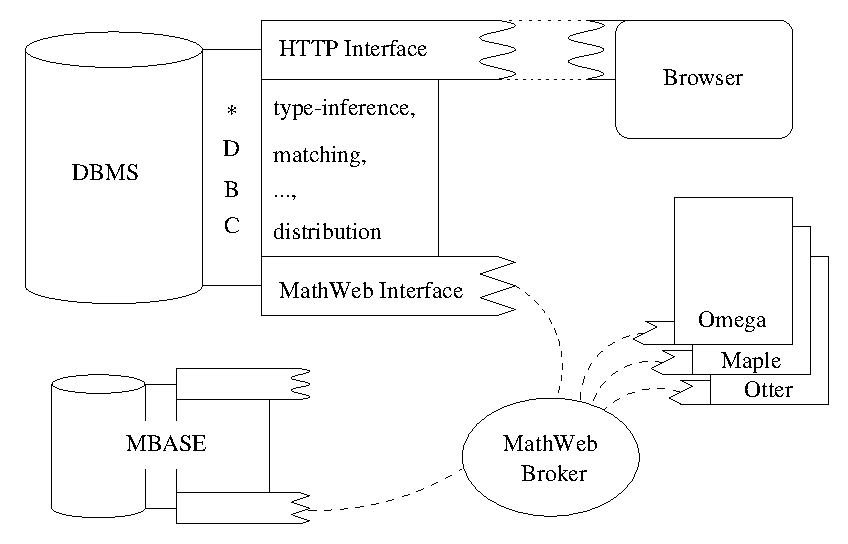
\includegraphics[width=10cm]{\projectsPath{mbase/mbase}}
    \caption{System Architecture}\label{fig:mbase}
  \end{center}
\end{figure}

{\mbase} supports transparent distribution of data among several {\mbase} servers
(see~\cite{KohFra:rkcimss01} for details). In particular, an object $O$ residing on an
{\mbase} server $S$ can refer to (or depend on) an object $O'$ residing on a server $S'$;
a query to $O$ that needs information about $O'$ will be delegated to a suitable query to
the server $S'$.  We distinguish two kinds of {\mbase} servers depending on the data they
contain: {\emph{archive servers}} contain data that is referred to by other {\mbase}s, and
{\emph{scratch-pad}} {\mbase}s that are not referred to. To facilitate caching protocols,
{\mbase} forces archive servers to be {\emph{conservative}}, i.e. only such changes to the
data are allowed, that the induced change on the corresponding logical theory is a
conservative extension.  This requirement is not a grave restriction: in this model errors
are corrected by creating new theories (with similar presentations) shadowing the
erroneous ones.  Note that this restriction does not apply to the non-logical data, such
as presentation or description information, or to scratchpad {\mbase}s making them ideal
repositories for private development of mathematical theories, which can be submitted and
moved to archive {\mbase}s once they have stabilized.
\end{omgroup}
%%% Local Variables: 
%%% mode: latex
%%% TeX-master: "../main"
%%% End: 

% LocalWords:  MBase mbase Franke Qed RDBMS http mbase
